\documentclass[aspectratio=1610]{beamer}

\usepackage{./util/zariski}

\usepackage{csquotes}
\usepackage{tikz}
\usepackage{tikz-cd}

\usetheme{Hannover}
% \usecolortheme{crane}
\setbeamertemplate{navigation symbols}{}

\author{Matthias Hutzler}
\title[Synthetic Algebraic Geometry]{Introduction to\\Synthetic Algebraic Geometry}
\date{Proof and Computation 2023\\Herrsching}


\begin{document}

\begin{frame}
  \maketitle
\end{frame}

\part{Lecture 1}

\section{Overview}

\begin{frame}
  \frametitle{What is synthetic algebraic geometry?}

  \begin{columns}[c]
    \begin{column}{0.2\textwidth}
    \end{column}
    \begin{column}{0.3\textwidth}
%      \flushright{$X^3 + X^2 - Y^2 = 0$}
      \[ X^3 + X^2 - Y^2 = 0 \]
    \end{column}
    \begin{column}{0.3\textwidth}
      \[
\begin{tikzpicture}[scale=1.5,domain=-1.0:0.8,samples=101]
        \draw[very thin,color=lightgray,step=0.5] (-1.1,-1.1) grid (1.1,1.1);
        \draw plot (\x,{ sqrt(abs(\x*\x + \x*\x*\x))});
        \draw plot (\x,{-sqrt(abs(\x*\x + \x*\x*\x))});
      \end{tikzpicture}\]
    \end{column}
    \begin{column}{0.2\textwidth}
    \end{column}
  \end{columns}

  \bigskip
  \begin{description}[synthetic algebraic geometry]
    \item[algebraic geometry]
      Thinking about algebra in geometric terms.
    \item<2->[synthetic algebraic geometry]
      Thinking about algebra in geometric terms,\\
      using a \alert{special language} that makes complex constructions look simple.
  \end{description}

  \bigskip
  \uncover<2->{\begin{itemize}
    \item
      language: homotopy type theory (HoTT) + three special axioms
    \item
      model: Zariski $\infty$-topos
  \end{itemize}}
\end{frame}

\begin{frame}
  \frametitle{What is synthetic algebraic geometry?}

  \center%
  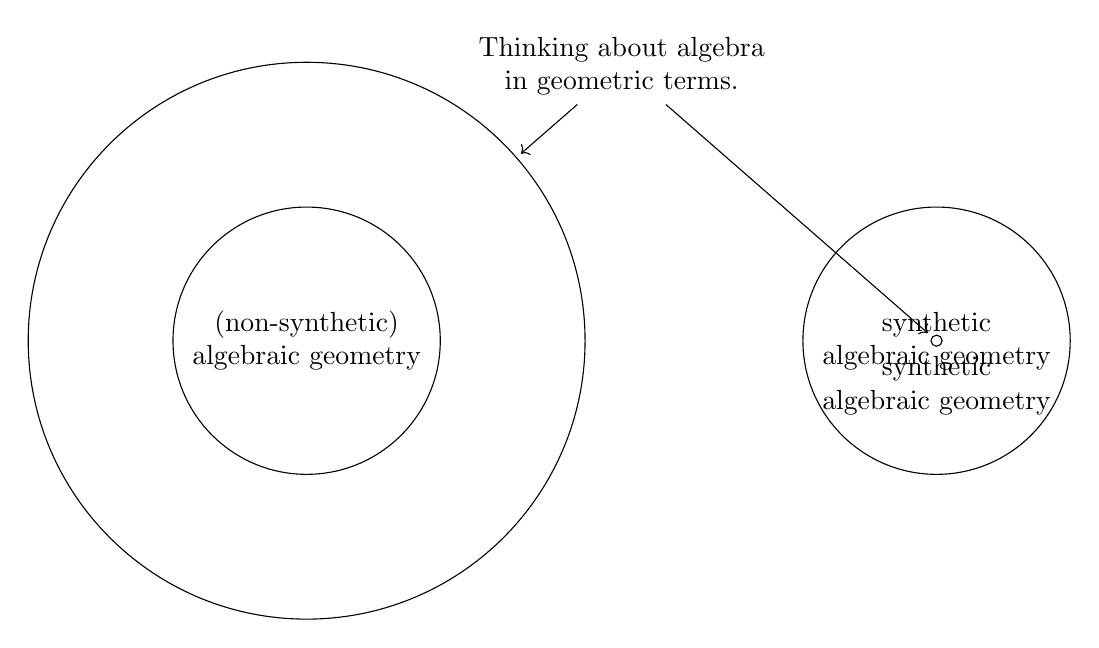
\begin{tikzpicture}
    % need align=* for line breaks
    \node[above,align=center] at (0,0) (start) {Thinking about algebra\\in geometric terms.};

    \node<1>[circle,draw,inner sep=1.2cm] at (-4,-3) (left) {};
    \node<2>[circle,draw,inner sep=2.5cm] at (-4,-3) (left) {};
    \node[align=center] at (left) {(non-synthetic)\\algebraic geometry};
    \node<1>[circle,draw,inner sep=1.2cm] at (4,-3) (right) {};
    \node<2>[circle,draw,inner sep=0.05cm] at (4,-3) (right) {};
    \node<1>[align=center] at (right) {synthetic\\algebraic geometry};
    \path<2> (right.south) node[below,align=center]{synthetic\\algebraic geometry};

    \draw[->,shorten >=2pt] (start) -- (left);
    \draw[->,shorten >=2pt] (start) -- (right);
  \end{tikzpicture}
\end{frame}

\begin{frame}
  \frametitle{Current work (since 2022)}

  \begin{block}{Preprint}
    F. Cherubini, T. Coquand, M. Hutzler,
    \textit{A Foundation for Synthetic Algebraic Geometry}\\
    \url{https://arxiv.org/abs/2307.00073}
  \end{block}

  \begin{block}{Computer formalization}
    in cubical Agda, very very incomplete\\
    \url{https://github.com/felixwellen/synthetic-geometry}
  \end{block}

  \begin{block}{Some people involved}
    Peter Arndt,
    Ingo Blechschmidt,
    Felix Cherubini,
    Thierry Coquand,
    Matthias Hutzler,
    Hugo Moeneclaey,
    David Jaz Myers,
    Marc Nieper-Wißkirchen,
    David Wärn,
    \dots
  \end{block}

  \begin{block}{Next workshop}
    2023-10-02 -- 2023-10-06, Augsburg\\
    \url{https://felix-cherubini.de/sag-meeting-3.html}
  \end{block}
\end{frame}

\begin{frame}
  \frametitle{Why \alert{you} might be interested}

  \begin{itemize}
    \item
      apply constructive reasoning
    \item
      apply homotopy type theory
    \item
      understand some algebraic geometry
    \item
      philosophically interesting phenomena
  \end{itemize}

  \bigskip
  \bigskip
  \center{\textit{Ask questions any time!}}
\end{frame}

\section{The spectrum of an algebra}

\begin{frame}
  \frametitle{Review of algebra}

  \begin{description}
    \item[ring]
      a set $R$ with $0, 1 : R$ and ${+}, {\cdot} : R \times R \to R$ such that:
      \begin{itemize}
        \item
          $+$ and $\cdot$ are associative, commutative, with unit $0$ resp.\ $1$
        \item
          $\cdot$ distributes over $+$
      \end{itemize}
      {\usebeamercolor[fg]{example text}
      e.g.\ %
      $\mathbb{Z}$,
      $\mathbb{R}$,
      $\mathbb{C}$,
      $\mathbb{Z}/(4)$,
      $\mathbb{C}[X]$,
      $\mathbb{C}[X, Y, Z]$,
      \dots}
      \pause%
    \item[$R$-algebra]
      a ring $A$ equipped with a ring homomorphism $R \to A$\\
      {\usebeamercolor[fg]{example text}
      e.g.\ %
      $R$,
      $R[X]$,
      $R/(r)$,
      $R[X, Y]/(X^3 + X^2 - Y^2)$,
      \dots}
  \end{description}

  \pause%
  \bigskip
  \bigskip
  An $R$-algebra $A$ is \emph{finitely presented} if:
  \[ A = R[X_1, \dots, X_n]/(p_1, \dots, p_m) \rlap{.}\]
\end{frame}

\begin{frame}<1>[label=DefSpec]
  \frametitle{Definition of the spectrum}

  \begin{columns}
    \begin{column}{0.5\textwidth}
      \begin{definition}[preliminary]
        For $P_1, \dots, P_m : R[X_1, \dots, X_n]$ define:
        \[
          \Spec\left(\begin{aligned}
            P_1 &= 0\\
            &\vdots\\
            P_m &= 0\\
          \end{aligned}\right)
          :=
          \{x : R^n \mid P_i(x) = 0\}
        \]
      \end{definition}
      \begin{example}
        $\Spec\Big(\,X - 1 = 0\,\Big) = \{1\}$
      \end{example}
    \end{column}

    \pause%
    \begin{column}{0.5\textwidth}
      \begin{definition}
        For a finitely presented $R$-algebra $A$ define:
        \[ \Spec(A) := \Hom_{\Alg{R}}(A, R) \]
      \end{definition}
      \begin{example}
        $\Spec(R[X]/(X - 1)) = \{f\}$,\\
        where $f(X) = 1$.
      \end{example}
    \end{column}
  \end{columns}
\end{frame}

\begin{frame}
  \frametitle{How are these systems of equations related?}

  \begin{columns}
    \begin{column}{0.25\textwidth}
      \[\begin{cases}
        X^2 + 1 = 0\\
      \end{cases}\]
    \end{column}
    \begin{column}{0.25\textwidth}
      \[\begin{cases}
        X^2 + 1 = 0\\
        X^3 + X = 0\\
      \end{cases}\]
    \end{column}
    \begin{column}{0.25\textwidth}
      \[\begin{cases}
        X^2 + 1 = 0\\
        Y = 0\\
      \end{cases}\]
    \end{column}
    \begin{column}{0.25\textwidth}
      \[\begin{cases}
        Y^2 + 1 = 0\\
        X = 0\\
      \end{cases}\]
    \end{column}
  \end{columns}
  \pause%
  \begin{columns}
    \begin{column}{0.25\textwidth}
      \[ R[X]/(X^2+1) \]
      \[\]
    \end{column}
    \begin{column}{0.25\textwidth}
      \[\]
      \[ R[X]/(X^2+1, X^3+X) \]
    \end{column}
    \begin{column}{0.25\textwidth}
      \[ R[X, Y]/(X^2+1, Y) \]
      \[\]
    \end{column}
    \begin{column}{0.25\textwidth}
      \[\]
      \[ R[X, Y]/(Y^2+1, X) \]
    \end{column}
  \end{columns}

  \bigskip
  \bigskip
  These $R$-algebras are all isomorphic.
\end{frame}

\againframe<2>{DefSpec}

\begin{frame}
  \[ \Spec(A) := \Hom_{\Alg{R}}(A, R) \]

  \bigskip
  \begin{example}
    \begin{itemize}
      \item
        $\Spec(R) = \pause \{*\}$
      \pause\item
        $\Spec(R[X]) = \pause R \quad$ (as a set)
      \pause\item
        $\Spec(R[X_1, \dots, X_n]) = \pause R^n$
      \pause\item
        $\Spec(R/(a)) = \pause \{* \mid a = 0\}$
      \pause\item
        $\Spec(R[a^{-1}]) = \pause \{* \mid \text{$a$ is invertible}\}$
    \end{itemize}
  \end{example}
\end{frame}

\begin{frame}
  \frametitle{Does $\Spec(A)$ faithfully represent $A$?}
  Let $R = \mathbb{Q}$.

  \[ \Spec(\mathbb{Q}[X]/(X)) = \{0\} = \Spec(\mathbb{Q}[X]/(X^2))\]

  \bigskip
  But the algebras are not isomorphic:
  \begin{itemize}
    \item
      $\mathbb{Q}[X]/(X) \cong \mathbb{Q}$
    \item
      $\mathbb{Q}[X]/(X^2) = \{ aX + b \mid a, b : \mathbb{Q}\}$
  \end{itemize}
\end{frame}

\begin{frame}
  \frametitle{Understanding algebraic subtleties geometrically}

  How is $X = 0$ different from $X^2 = 0$ geometrically?
  \bigskip

  \begin{columns}<2->
    \begin{column}{.5\textwidth}
      \[\begin{cases}
        X = 0 \\
        Y = 0
      \end{cases}\]
      \center%
      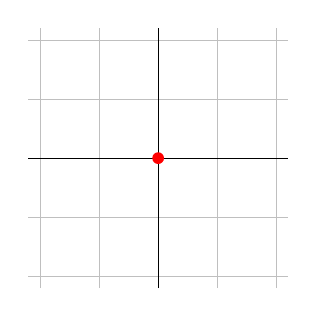
\begin{tikzpicture}[scale=1.5,domain=-1.1:1.1]
        \draw[very thin,color=lightgray,step=0.5] (-1.1,-1.1) grid (1.1,1.1);
        \draw plot (0,\x);
        \draw plot (\x,0);
        \path<3-> (0,0) node[red,circle,fill,inner sep=1.5pt]{};
      \end{tikzpicture}
      \center%
      \uncover<3->{a point}
    \end{column}
    \begin{column}{.5\textwidth}
      \[\begin{cases}
        X^2 - Y = 0 \\
        Y = 0
      \end{cases}\]
      \center%
      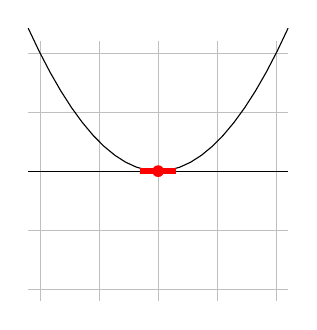
\begin{tikzpicture}[scale=1.5,domain=-1.1:1.1]
        \draw[very thin,color=lightgray,step=0.5] (-1.1,-1.1) grid (1.1,1.1);
        \draw plot (\x,\x*\x);
        \draw plot (\x,0);
        \path<3-> (0,0) node[red,circle,fill,inner sep=1.5pt]{};
        \draw<3->[red,line width=2pt] (-0.15,0) -- (0.15,0);
      \end{tikzpicture}
      \center%
      \uncover<3->{an \enquote{infinitesimally thickened} point}
    \end{column}
  \end{columns}
\end{frame}

\section{The first two axioms}

\begin{frame}
  \frametitle{The first axiom (Loc)}

  \[ \Spec(\;R[X]/(X\cdot(X-1))\;) = \text{?} \]

  \pause%
  \bigskip
  \begin{block}{Axiom (Loc)}
    $R$ is a \emph{local} ring.
    That is:
    \begin{itemize}
      \item
        $0 \neq 1$
      \item
        For every $x : R$,
        $x$ is invertible or $1 - x$ is invertible.
    \end{itemize}
  \end{block}

  \bigskip
  With (Loc) we have:
  \[ \Spec(\;R[X]/(X\cdot(X-1))\;) = \{0, 1\} \]
  \pause%
  and also:
  \[ \Spec(\;R[X]/((X-a_1)\cdot \dots \cdot(X-a_n))\;) = \{a_1, \dots, a_n\} \]
  if all $a_i - a_j$ are invertible.
\end{frame}

\begin{frame}[fragile] % fragile for tikzcd
  \frametitle{The axiom of synthetic quasi-coherence (SQC)}
  \begin{block}{Axiom (SQC)}
    For every finitely presented $R$-algebra $A$,
    the map
    \[\begin{tikzcd}[row sep=0pt]
      A \ar[r] & R^{\Spec(A)} \\
      a \ar[r, mapsto] & (\varphi \mapsto \varphi(a))
    \end{tikzcd}\]
    is bijective.
  \end{block}
\end{frame}

\begin{frame}
  \frametitle{First consequences}
\end{frame}

\part{Lecture 2}

\section{Schemes}

\begin{frame}
  \frametitle{Affine schemes}
\end{frame}

\begin{frame}
  \frametitle{Motivation for non-affine schemes}

  \begin{example}
    The two equations

    are equivalent:
  \end{example}

  We want to consider the space of all \alert{ratios} $[x : y : z]$
  for $x, y, z : R$.
\end{frame}

\begin{frame}
  \frametitle{Definition of scheme}
\end{frame}

\section{Line bundles}

\begin{frame}
  \frametitle{Line bundles}
\end{frame}

\section{Computer formalization}

\begin{frame}
  \frametitle{
\includegraphics[width=5cm]{./images/agda-logo.png}}

  Agda is
  \begin{itemize}
    \item
      a functional programming language
      \begin{itemize}
        \item
          influenced by Haskell
      \end{itemize}
    \item
      a proof assistant
      \begin{itemize}
        \item
          with a \alert{cubical type theory} mode
      \end{itemize}
  \end{itemize}
\end{frame}

\begin{frame}
  \frametitle{Tangent space}
\end{frame}

\end{document}
